\documentclass[dvipsnames,hidelinks]{beamer}

  % Enables the use of colour.
  \usepackage{xcolor}
  % Syntax high-lighting for code. Requires Python's pygments.
  \usepackage{minted}
  % Enables the use of umlauts and other accents.
  \usepackage[utf8]{inputenc}
  % Diagrams.
  \usepackage{tikz}
  % Settings for captions, such as sideways captions.
  \usepackage{caption}
  % Symbols for units, like degrees and ohms.
  \usepackage{gensymb}
  % Latin modern fonts - better looking than the defaults.
  \usepackage{lmodern}
  % Allows for columns spanning multiple rows in tables.
  \usepackage{multirow}
  % Better looking tables, including nicer borders.
  \usepackage{booktabs}
  % More math symbols.
  \usepackage{amssymb}
  % More math fonts, like mathbb.
  \usepackage{amsfonts}
  % More math layouts, equation arrays, etc.
  \usepackage{amsmath}
  % More theorem environments.
  \usepackage{amsthm}
  % More column formats for tables.
  \usepackage{array}
  % Adjust the sizes of box environments.
  \usepackage{adjustbox}
  % Better looking single quotes in verbatim and minted environments.
  \usepackage{upquote}
  % Better blank space decisions.
  \usepackage{xspace}
  % Better looking tikz trees.
  \usepackage{forest}
  % URLs.
  \usepackage{hyperref}
  % For plotting.
  \usepackage{pgfplots}
  % For more font sizes.
  \usepackage{anyfontsize}
  
  % Various tikz libraries.
  % For drawing mind maps.
  \usetikzlibrary{mindmap}
  % For adding shadows.
  \usetikzlibrary{shadows}
  % Extra arrows tips.
  \usetikzlibrary{arrows.meta}
  % Old arrows.
  \usetikzlibrary{arrows}
  % Automata.
  \usetikzlibrary{automata}
  % For more positioning options.
  \usetikzlibrary{positioning}
  % Creating chains of nodes on a line.
  \usetikzlibrary{chains}
  % Fitting node to contain set of coordinates.
  \usetikzlibrary{fit}
  % Extra shapes for drawing.
  \usetikzlibrary{shapes}
  % For markings on paths.
  \usetikzlibrary{decorations.markings}
  % For advanced calculations.
  \usetikzlibrary{calc}
  
  % GMIT colours.
  \definecolor{gmitblue}{RGB}{20,134,225}
  \definecolor{gmitred}{RGB}{220,20,60} 
  \definecolor{gmitgrey}{RGB}{67,67,67}
  
  % Change some style options.
  \usetheme{metropolis}
  % Tell minted to use the following colour scheme. 
  \usemintedstyle{manni}

  \metroset{sectionpage=simple, numbering=none, block=fill}

  % Change the default theme colours.
  \setbeamercolor{normal text}{fg=darkgray, bg=white}
  \setbeamercolor{alerted text}{fg=gmitred, bg=white}
  \setbeamercolor{example text}{fg=gmitblue, bg=white}
  \setbeamercolor{frametitle}{fg=white, bg=gmitblue}
  \setbeamercolor*{item}{fg=gmitblue}
  % Use a better math mode font.
  \usefonttheme[onlymath]{serif}

  % \citeurl can be used to a clickable short url to a slide as a reference.
  \renewcommand\footnoterule{}
  \newcommand{\citeurl}[1]{\let\thefootnote\relax\footnotetext{\tiny \textcolor{gmitgrey}{\href{http://#1}{#1}}}}
  \newcommand{\citeeg}[1]{\let\thefootnote\relax\footnotetext{\tiny \textcolor{gmitgrey}{#1}}}
  
  % Prevent minted from showing errors.
  \makeatletter
  \expandafter\def\csname PYGdefault@tok@err\endcsname{\def\PYGdefault@bc##1{{\strut ##1}}}
  \makeatother
  
  \setbeamertemplate{section page}
  {
      \begin{centering}
      \begin{beamercolorbox}[sep=12pt,center]{part title}
      \usebeamerfont{section title}\insertsection\par
      \end{beamercolorbox}
      \end{centering}

      \begin{center}
        \small ian.mcloughlin@gmit.ie
      \end{center}
  } 


\begin{document}
  \section{The Square Root of 2}

\begin{frame}
  \begin{columns}
    \begin{column}{0.3\textwidth}
      \centering
      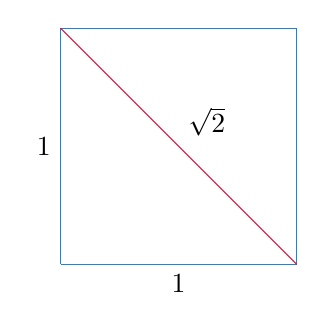
\begin{tikzpicture}
        \draw[draw=gmitblue] (0,0) --node [midway, left, black] {$1$} (0,3) -- (3,3) -- (3,0) --node [midway, below, black] {$1$} (0,0);
        \draw[gmitred] (3,0) -- (0,3) node [midway, above right, black] {$\sqrt{2}$};
      \end{tikzpicture}
    \end{column}
    {\color{gmitgrey!30}\vrule{}} \hspace{0.1\textwidth}
    \begin{column}{0.5\textwidth}
      $\sqrt{2} \times \sqrt{2} = 2$ \\[8mm]
      $d^2 = \sqrt{l^2 + w^2}$ \\[8mm]
      $d^2 = \sqrt{1^2 + 1^2}$ \\[8mm]
      $d^2 = \sqrt{2}$ \\[8mm]
    \end{column}
  \end{columns}
\end{frame}


\begin{frame}
  \begin{columns}
    \begin{column}{0.3\textwidth}
      \color{gmitblue} \fontsize{30}{10}
      \[\frac{a}{b}\]
    \end{column}
    {\color{gmitgrey!30}\vrule{}} \hspace{0.1\textwidth}
    \begin{column}{0.5\textwidth}
      $\sqrt{2} = \dfrac{a}{b}$ \\[8mm]
      $\Rightarrow 2 = \dfrac{a^2}{b^2}$ \\[8mm]
      $\Rightarrow 2b^2 = a^2$ \\[8mm]
      $\Rightarrow 2 \mid a^2$ \\[8mm]
      $\Rightarrow 2 \mid a$
    \end{column}
  \end{columns}
\end{frame}


\begin{frame}
  \begin{columns}
    \begin{column}{0.3\textwidth}
      \color{gmitblue} \fontsize{30}{10}
      \[2 \mid a\]
    \end{column}
    {\color{gmitgrey!30}\vrule{}} \hspace{0.1\textwidth}
    \begin{column}{0.5\textwidth}
      $2 \mid a$ \\[8mm]
      $\Rightarrow 4 \mid a^2$ \\[8mm]
      $\Rightarrow 4 \mid 2b^2$ \\[8mm]
      $\Rightarrow 2 \mid b^2$ \\[8mm]
      $\Rightarrow 2 \mid b$
    \end{column}
  \end{columns}
\end{frame} 
\end{document}